%! Author = cspiller
%! Date = 17/11/2022

\thispagestyle{plain}
\newpage
\section{Literature Review}\label{sec:literature-review}

\normalsize

As outlined in~\ref{subsec:aims}, this project attempts to engage with cloud infrastructure, spatial audio processing, and web development frameworks.
To approach these topics thoroughly, this report performs a review of pertinent literature.
In doing so, this report considers and incorporates existing ideas in these fields while providing a foundation from which to answer the research questions listed in~\ref{subsec:research-questions}.

\subsection{Cloud Computing}\label{subsec:cloud-computing}

Ever since internet service providers began the commercialization of cloud computing,
it has become one of the major trends in the technology industry~\citep{cc_overview}.
According to~\citet{cc_overview}, `cloud computing' is one of the most vague terms when it comes to the description of the technology.
This is because of the breadth of functions it encompasses.
The US National Institute of Standards and Technology (NIST) clarify:

\begin{quotation}
    ``Cloud computing is a model for enabling ubiquitous, convenient, on-demand network access to a shared pool of configurable computing resources (e.g., networks, servers, storage, applications, and services) that can be rapidly provisioned and released with minimal management effort or service provider interaction.''~\citep{mell2011nist}
\end{quotation}\citet{mell2011nist} and~\citet{marinescu-cloud} go on to identify key characteristics of cloud computing:

\begin{enumerate}
    \item On-demand self-service: a user can provision computing resources without needing human assistance
    \item Broad network access: the ability to provision resources can be accessed using the internet and through `normal' devices such as computers or mobile phones
    \item Resource pooling: the provider of cloud services dynamically assigns resources to multiple customers in accordance with demand; the exact physical location of these resources are not revealed to the customer but can be narrowed down to the datacenter or accessibility zone in which multiple resources are held for use
    \item Rapid elasticity: provisioning and de-provisioning of resources occurs automatically and gives the appearance of unlimited resources to the consumer
    \item Measured service: both the provider and consumer of the cloud services are able to monitor its usage for optimization and cost management purposes
\end{enumerate}

The ethos behind cloud computing systems is that data processing and storage can be done more efficiently, and be more cost-effective, as a part of large `farms' of computing systems~\citep{marinescu-cloud}.
Cloud computing has gained popularity in enterprise because of the benefits it provides,
such as reduced cost (compared to on-premises computing services), pay-as-you-go pricing, on-demand elasticity,
and not needing to worry about hardware implementation and maintenance~\citep{kumar-cloud}.

However, as~\citet{cc_challenges} note,
cloud computing in its early stages of development and adoption stage was associated with different challenges,
 especially in enterprise contexts.
Figure~\ref{fig:cloud-challenges} shows the results from an IDC Survey conducted in 2009.
The survey asked organisations about what challenges prevented the adoption of cloud computing.
While many of these concerns have been addressed in the intervening years since the survey,
the challenges raised in the survey are still of relevance, most notably that of security, cost, and vendor locking
(not being able to migrate services out of the cloud because of a lack of interoperability standards).
In addition, the ethics of any new technology should also be considered.

\begin{figure}[!htb]
    \centering
    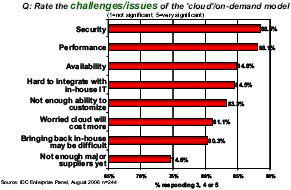
\includegraphics[width=9cm]{cloud-challenges}
    \caption{Cloud adoption challenges survey. Taken from~\citep{cloud-survey}.}\label{fig:cloud-challenges}
\end{figure}

The paper by~\citet{timmermans2010ethics} addresses some of the ethical concerns of cloud computing.
Ethical issues can derive from the following three characteristics of cloud computing:

\begin{itemize}
    \item Shifting control from technology users to third parties
    \item Storage of data in multiple physical locations around the world, and administrated by different organisations
    \item The interconnection of multiple services across the cloud
\end{itemize}

Issues of data ownership, privacy, disaster recovery,
and accountability become complicated in the ceding of control to third parties when using cloud computing services~\citep{timmermans2010ethics}.
\citet{ess_2008} also notes that cloud computing touches on issues of cultural imperialism due to the fact
that the majority of cloud providers will originate from western cultures, in particular, from the US\@.
This may lead to the imposition of western ideals into cloud frameworks and regulations,
leading to cultural homogenization and the suppressing of local cultures.
While~\citet{timmermans2010ethics} doesn't contain any explicit recommendations to ameliorate these matters,
recommendations are made to utilise information technology governance in the integration of ethics into software development.

Legal issues, particularly concerning~\gls{ip} have been identified by~\citet{roszell_baker_2020}.
The cloud can be the cause of complications for~\gls{ip} holders in that cloud technology is cross-jurisdictional
(where does infringement occur?),
has multi-party operation (who caused the infringement?), and obfuscatory (how I can detect when infringement occurs?).
Each of these characteristics provides reason for pause for those
looking to protect their~\gls{ip} or for those looking to store potentially copyrighted material.
Furthermore,~\citet{roszell_baker_2020} recommends
that businesses looking to use cloud technology should prepare and plan for such issues in the way
they architect their cloud solutions.

Today public cloud computing technology is dominated by three major players, each with their own style of cloud services:

\begin{enumerate}
    \item Amazon's Web Services which began as a means of server virtualization~\citep{awsintro}
    \item Google's Cloud Platform, described by~\citet{cc_overview} as a technique-specific sandbox that calls itself a~\gls{paas}~\citep{googlecloudintro}
    \item Microsoft's Azure Network~\citep{azurefundamentals}
\end{enumerate}

While these are the `big three' of service providers, the public cloud market is expanding with other smaller providers offering their own low-cost services.

\citet{weinman2012cloudonomics}\('\)s book,~\textit{\usebibentry{weinman2012cloudonomics}{title}}, identifies the ways in which businesses are able to leverage cloud services but also highlights how the benefit of the technology will be individual to the organisation and their goals.
Companies can use the cloud to increase the availability of their services and data,
with uptime being a key metric that is linked to revenue~\citep{weinman2012cloudonomics}.
It can also increase the agility of companies whereby new services and resource requirements can be spun up in response to changing business needs,
without the overhead costs of new data centres and hardware.
\citet{weinman2012cloudonomics} also notes the following:

\begin{quotation}
    Revenue growth can be enhanced via the cloud, through:
    \begin{itemize}
        \item Greater value incorporated into the product or service
        \item Greater market penetration through the global reach of the cloud
        \item Greater availability through replication of data and application resources
        \item Greater conversion of sales through scalable online channel resources
        \item Greater customer engagement through richer experiences delivered via the cloud
        \item Greater revenue, allowing for the time value of money, by accelerating future revenue streams into the present
    \end{itemize}~\citep{weinman2012cloudonomics}
\end{quotation}

Cloud computing also provides benefits in terms of hardware standardisation and performance~\citep{rehr_scientific}.
Some workloads, especially in the scientific domain, require significant amounts of computing power.
Cloud services such as~\gls{aws} provide the framework
for provisioning high-capacity computer resources with the potential
for setting up parallel computing to increase performance for intensive workloads~\citep{rehr_scientific}.

\subsection{Audio Spatialisation}\label{subsec:audio-spatialisation}
\subsubsection{Origins}

A patent filed in 1958 by Alan Dower Blumlein detailed an early stereophonic system, which exploited the human sound localization ability for the enhancement of entertainment experiences\footnote{This report acknowledges that this is not the first example of this kind of system; the control of inter-aural time differences was pioneered by Cl\'ement Ader as early at 4 years after Bell's invention of the telephone. This was for the purpose of rendering a spatial transmission of the Paris Opera. This further solidifies a history of the desire for spatial immersion in entertainment.}\footnote{There is a rich history of considering space in the composition of music in Western Classical tradition, with Italian renaissance composers writing for \textit{cori spezzati}, or multiple choirs that are spatially separated~\citep{spezzati}. Unfortunately the topic of spatialisation in historic acoustic performance goes beyond the scope of this report.}~\citep{blumlein-patent}.
Blumlein observed that in film theatres there existed a certain level of cognitive dissonance whereby the actor’s voices sounded like they were coming from a different location than where they appeared on the screen~\citep{alexander_blumlein}.
This patent, in response,
specifically outlines methods for introducing stereophonic audio to sound film as a means
of increasing the perceived `quality' of the entertainment experience.
Blumlein acknowledges that human binaural hearing is responsible for the ability to localize sound, and his patent is an example of how one might induce an auditory event that exhibits spatialisation on the horizontal plane through the control of inter-aural time differences~\citep{blumlein-patent}.

The patent marked an improvement in the way that auditory events might be replicated by introducing this form of spatialisation, and the vestiges of Blumlein`s ideas can be observed in modern spatial audio techniques~\citep{spatial_techniques, beyer_acoustics}.
What is perhaps the most salient aspect of the patent, however, is that it recognizes the physiological factors that are involved in human sound localization.
These physiological factors explored and expounded upon by~\citet{blauert_spatial}, and, as noted in the 1996 revision of his book, become more important as audio spatialisation and entertainment technology attempt to induce auditory events that imply three-dimensional audio spaces.

\subsubsection{From two to three}

\begin{quotation}
    The external ears superimpose linear distortions on the incoming signals, which, in each case, are specific for the direction of incidence of the sound wave and the source distance.
    In this way, spatial information is encoded into the signals that are received by the eardrums~\citep{blauert_spatial}.
\end{quotation}

\citet{roginska2017immersive} note that:~\textquote{the word `binaural' refers, at the most basic level, to hearing with two ears, but it later came to include all the spatial cues from the ears, head, and body of a listener}.
Binaural recordings can therefore refer to the practice of capturing sounds that incorporate human physiology.
This is executed with test double mannikin heads with microphones placed inside the ears so that sound entering them is affected by the `blocking' nature of the head;
developments in this technology rapidly sped up throughout the 20th century~\citep{binaural_paul}.
While other forms of spatial representation were developed in this period~\citep{gerzon_periphony, noisternig_ambisonic, wave_field}, technology that considers the physical and physiological factors in human listening when attempting to induce auditory events that feature sound localization.

\citet{roginska2017immersive} identify that while capturing binaural audio is relatively easy, realizing the same effect through post-recording production is considerably harder and poses the challenge of modelling the human spatialization facility.

\subsubsection{Getting the head in the game}

The~\glsaccessfirst{hrtf} can be described as a representation of the perceptual cues that facilitate human sound localization as a sound propagates from its source to the human ear~\citep{Suzuki2011}.
This modelling of the human sound localization facility allows for this~\gls{hrtf} to be applied to a sound before reaching the human eardrum~\citep{roginska2017immersive}.
It is with this technology that more and more modern entertainment systems begin to localize sounds~\citep{blauert_spatial, HONDA2007, roginska2017immersive, Suzuki2011, Xie2013, ps5_audio, soundscape_design} during audio playback.

There are many software systems, toolkits, and frameworks that have been developed to allow engineers to build software that can utilise~\glspl{hrtf} and apply them to monophonic recordings~\citep{3d_tune_in, resonance}.
It is through these technologies that many video game systems such as the~\gls{ps5} are able to provide immersive~\gls{3d} audio experiences.
In commercial systems such as these, consideration must also be applied to the selection of the~\gls{hrtf} that are used.
While each person's experience of sound is as individual as they are, capturing the~\gls{hrtf} of each individual who engages with the product is not yet feasible due to the highly involved and costly process of capturing them.
Considerable research has been done in order to develop and produce~\gls{hrtf} databases that appeal to a wide variety of subjects, taking into account individual and non-individual~\glspl{hrtf}~\citep{armstrong_}.
It is common practice to have entertainment systems contain multiple~\gls{hrtf} options to choose from when setting up that system's spatial audio capabilities~\citep{shukla2018user}.

\subsection{Web interfaces}\label{subsec:web-interfaces}
\citet{kantamneni2022user} posits
that ``every company is now a technology company''
and that the technology products they offer must account for all users engaged in their business ecosystem.
Using the failed centralization of the UK's health records system as an example, the author argues
that not considering the user in the design of software systems can have dire ramifications on the success of any software project,
especially those which are intended to be used by customers of competitive organisations~\citet{kantamneni2022user}.

\citet{garrett2010elements} also observes that:

\begin{quotation}
    When a product is being developed, people pay a great deal of attention to what it does.
    User experience is the other, often overlooked, side of the equation—how it works—that can often make the difference between a successful product and a failure.
\end{quotation}

\citet{garrett2010elements} encourages the idea that design should have user experience as an explicit outcome,
and this means looking beyond only the functional and aesthetic.
In the case of producing audio-based applications,
a number of different techniques can be employed
to provide more immersive and intuitive representations of audio data~\citep{geolocation-player, discovery-collections}


\subsection{Web audio}\label{subsec:web-audio}

Audio-visual media on the internet is extremely widespread and can be delivered in many ways~\citep{Bruegger2018}.
The means by which audio is delivered to users on the internet is most frequently through a web audio~\gls{api}, the most common of which is the one developed by Mozilla~\citep{w3c_audio_api, mdn_audio_api}.
One of the major benefits of utilising web technology in combination with audio technology is that it allows developers and those who wish to present audio to an audience to do so with a rich toolset of graphical libraries that are easily accessed through a web browser~\citep{Pauwels2018pywebaudioplayerBT};
this is most frequently seen in commercial usage through web audio players such as Spotify and SoundCloud as natural evolution of the radio broadcasting format~\citep{Bottomley2020}.
Web frameworks such as React.js~\citep{Minnick2022}, Flask~\citep{Zhai2022},
and Django~\citep{Pauwels2018pywebaudioplayerBT} are all capable of handling and displaying audio representations from a web page.

Audio delivery is primarily executed through the downloading and playing of a static file or as a packet stream from a server-based audio file source;
however, more recently web audio can be delivered peer-to-peer in real-time through such technologies like WebRTC~\citep{webrtc, Garcia2019}.
